The Cosmic Microwave Background is the first electromagnetic signal we can study since the Big Bang. It thus encodes a wealth of cosmological information from the epoch of recombination (and reionization). In this study, we use data from the Planck satellite missjon [reference] to find the geometry of spacetime by studying this primordial signal.

\vspace{0.5em}
\begin{figure}
	\begin{minipage}{0.3\textwidth}
		\centering\includegraphics[width=1.1\textwidth]{poster_labyCMB/img/sphere.png}
	\end{minipage}
	\hspace{1em}
	\begin{minipage}{0.3\textwidth}
		\centering\includegraphics[width=1\textwidth]{poster_labyCMB/img/flat.png}
		\caption{Nullam pulvinar nulla quis felis posuere condimentum.}
	\end{minipage}
	\hspace{1em}
	\begin{minipage}{0.3\textwidth}
		\centering\includegraphics[width=1\textwidth]{poster_labyCMB/img/saddle.png}
	\end{minipage}
\end{figure}

According to General Relativity [ref], spacetime can feature three types of geometry: 

\vspace{0.4em}
\begin{figure}
\begin{minipage}{0.43\textwidth}
	\centering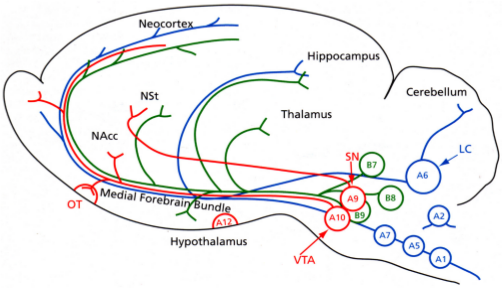
\includegraphics[width=0.85\textwidth]{img/mas.png}
	\caption{Lorem ipsum dolor sit amet \cite{Paivi}}
\end{minipage}
\hspace{1em}
\end{figure}

Ut dapibus est non condimentum laoreet. Curabitur mollis leo diam, nec sagittis lorem bibendum a. Curabitur efficitur ante consequat euismod imperdiet. Nam arcu lacus, luctus non porttitor at, eleifend sit amet leo. Phasellus volutpat, nibh nec porta volutpat, nisl sem cursus sapien, non molestie nisl ipsum et enim.